\newpage
\section*{CHAPTER 3. IMPLEMENTATION}
\phantomsection\addcontentsline{toc}{section}{CHAPTER 3. IMPLEMENTATION}
\setcounter{section}{3}
\setcounter{figure}{0}
\setcounter{subsection}{0}
\setcounter{subsubsection}{0}
\setcounter{paragraph}{0}
\setcounter{table}{0}

Chapter 3 presents the implementation of the proposed HiFiC GAN accelerator. Following the organization of a typical implementation chapter, the discussion begins with the system-level architecture and design flow, then focuses on the internal accelerator blocks, and finally describes how the design is prepared for deployment on the ZCU104 FPGA platform.

The goal of this chapter is not to redefine the HiFiC algorithm, which has already been introduced in the theoretical background, but to explain how the model is mapped into a practical hardware--software co-design. Therefore, the chapter emphasizes architectural partitioning, data movement, buffering, parallel computation, and the High-Level Synthesis (HLS) flow used to generate the FPGA accelerator.

%%%%%%%%%%%%%%%%%%%%%%%%%%%%%%%%%%%%%%%%%%%%%%%%%%%%%%%%%%%%%%%%%%%%%%%%%%%%%%%%%%%%%%%%%%%%%%%%%%%%
\subsection{System-Level Architecture Design}

\textbf{System specifications:}
\begin{itemize}
    \item Input data: RGB image with a resolution of $256 \times 256$.
    \item Target model: Quantized HiFiC GAN inference for learned image compression and reconstruction.
    \item Target platform: ZCU104 FPGA development board.
    \item Design tools: C/C++ for accelerator modeling, Vitis HLS for hardware synthesis, Vivado for system integration, and Vitis for software control on the embedded processor.
\end{itemize}

Figure~\ref{fig:flow_design} shows the overall implementation flow used in this project. The flow connects the software model, HLS accelerator design, FPGA system integration, and board-level execution into a single development process.

\begin{figure}[H]
    \centering
    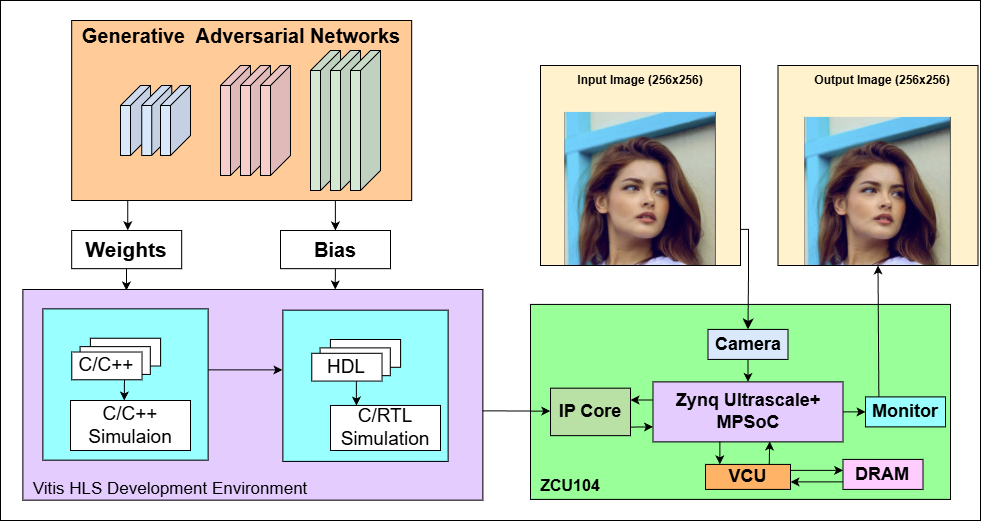
\includegraphics[width=\textwidth]{Images/Flow_design.png}
    \caption{Overall implementation flow of the HiFiC GAN accelerator}
    \label{fig:flow_design}
\end{figure}

The first stage analyzes the HiFiC inference pipeline and identifies the blocks that dominate computation. The model structure and parameters are then converted into a C/C++ implementation suitable for hardware synthesis. This C/C++ model is used as both the functional reference and the basis for the accelerator kernel.

The second stage uses Vitis HLS to synthesize the selected compute kernel into register-transfer level (RTL) hardware. During this step, loop pipelining, array partitioning, on-chip buffering, and interface directives are applied to expose parallelism and reduce unnecessary memory accesses. The generated RTL block is exported as an FPGA IP core.

The final stage integrates the IP core into a Zynq UltraScale+ system using Vivado. The accelerator is connected to external DDR memory and the Processing System (PS) through AXI interfaces. A Vitis software application configures the accelerator, transfers input data and parameters, starts execution, and collects output feature maps for the remaining stages of the image reconstruction pipeline.

\subsubsection{HiFiC GAN Model-Level Data Path}

This subsection first clarifies the model-level data path before discussing hardware partitioning. The purpose is to identify which part of the HiFiC inference pipeline should remain in software and which part should be mapped to the FPGA accelerator.

The overall HiFiC architecture used in this project is shown in Figure~\ref{fig:hific_overall}. The model consists of an encoder network, a hyperprior network, and a generator network. The encoder transforms the input image into a compact latent representation, while the hyperprior network provides side information for entropy modeling. The generator reconstructs the final image from the latent representation and is responsible for recovering high-quality visual details.

\begin{figure}[H]
    \centering
    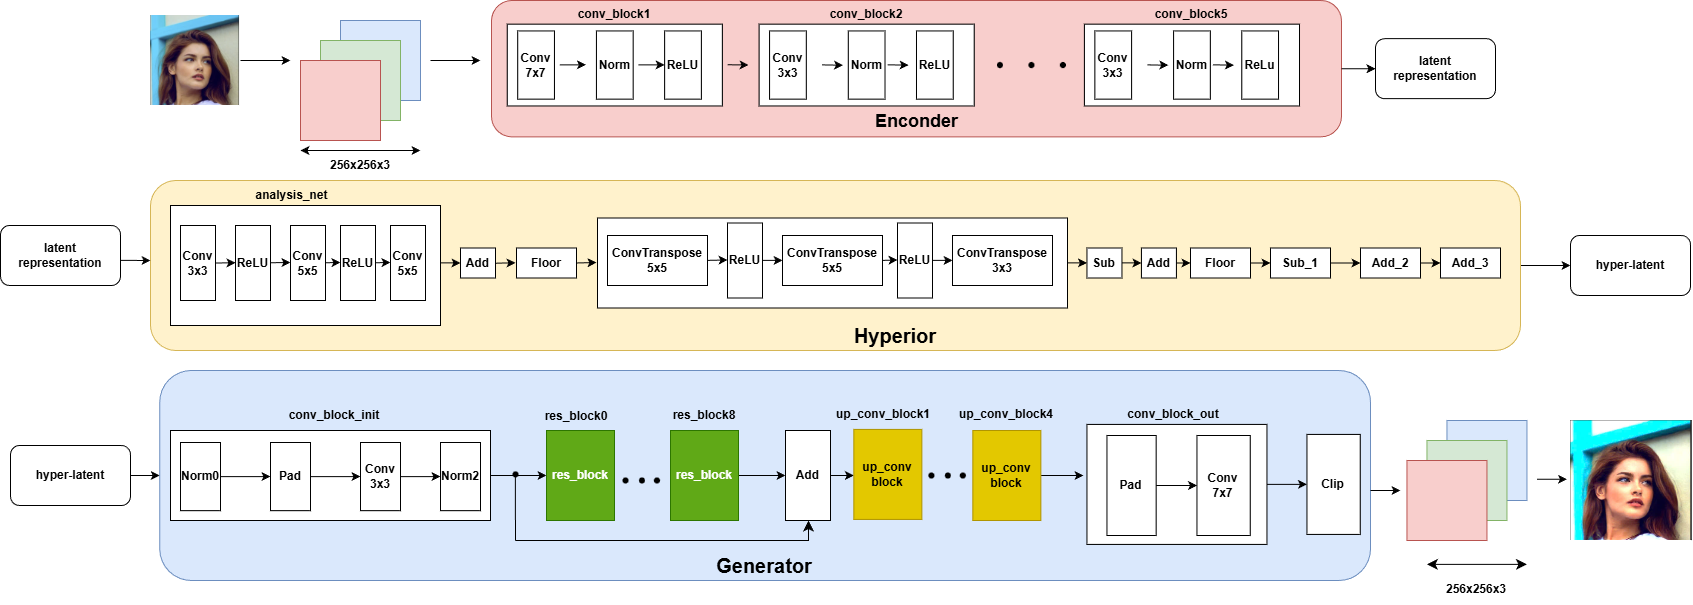
\includegraphics[width=0.9\textwidth]{Images/HiFiC.png}
    \caption{Overview of the HiFiC GAN-based learned image compression architecture}
    \label{fig:hific_overall}
\end{figure}

From the implementation perspective, the encoder and hyperprior mainly define the compression control path and model preparation flow, whereas the generator dominates reconstruction computation. As illustrated in Figure~\ref{fig:generator_structure}, the generator includes an initial convolution block, multiple residual blocks, several up-convolution blocks, and an output convolution block. The residual blocks are repeated many times and contain a large number of multiply--accumulate (MAC) operations, so they become the main candidate for FPGA acceleration.

\begin{figure}[H]
    \centering
    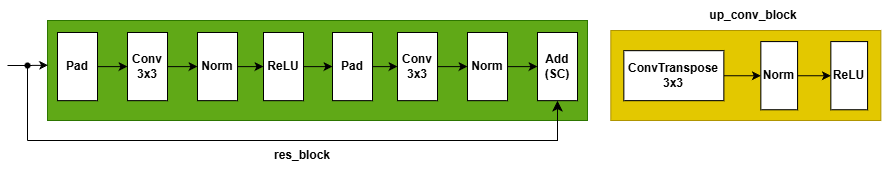
\includegraphics[width=0.9\textwidth]{Images/GAN.png}
    \caption{Generator structure with residual blocks and up-convolution blocks}
    \label{fig:generator_structure}
\end{figure}

Therefore, the system-level design decision is derived directly from the model data path: software preserves the flexible parts of the HiFiC pipeline, while hardware focuses on the repeated ResBlock computation inside the generator. This relationship is the basis for the hardware--software partitioning described next.

\subsubsection{System Partitioning and PS--PL Interfaces}

Based on the model-level analysis in the previous subsection, the proposed implementation follows a hardware--software co-design strategy. Tasks that require flexibility, irregular control, file handling, or model orchestration are executed on the Processing System (PS). The computationally intensive residual blocks are offloaded to the Programmable Logic (PL), where parallel datapaths and streaming buffers can be customized for the convolution workload.

Figure~\ref{fig:hw_sw_overview} summarizes this partitioning. The PS manages model control, parameter preparation, memory allocation, and accelerator invocation. The PL executes the ResBlock accelerator as a reusable compute kernel. Large tensors are exchanged through shared DDR memory, while lightweight control signals are transferred through memory-mapped AXI registers.

\begin{figure}[H]
    \centering
    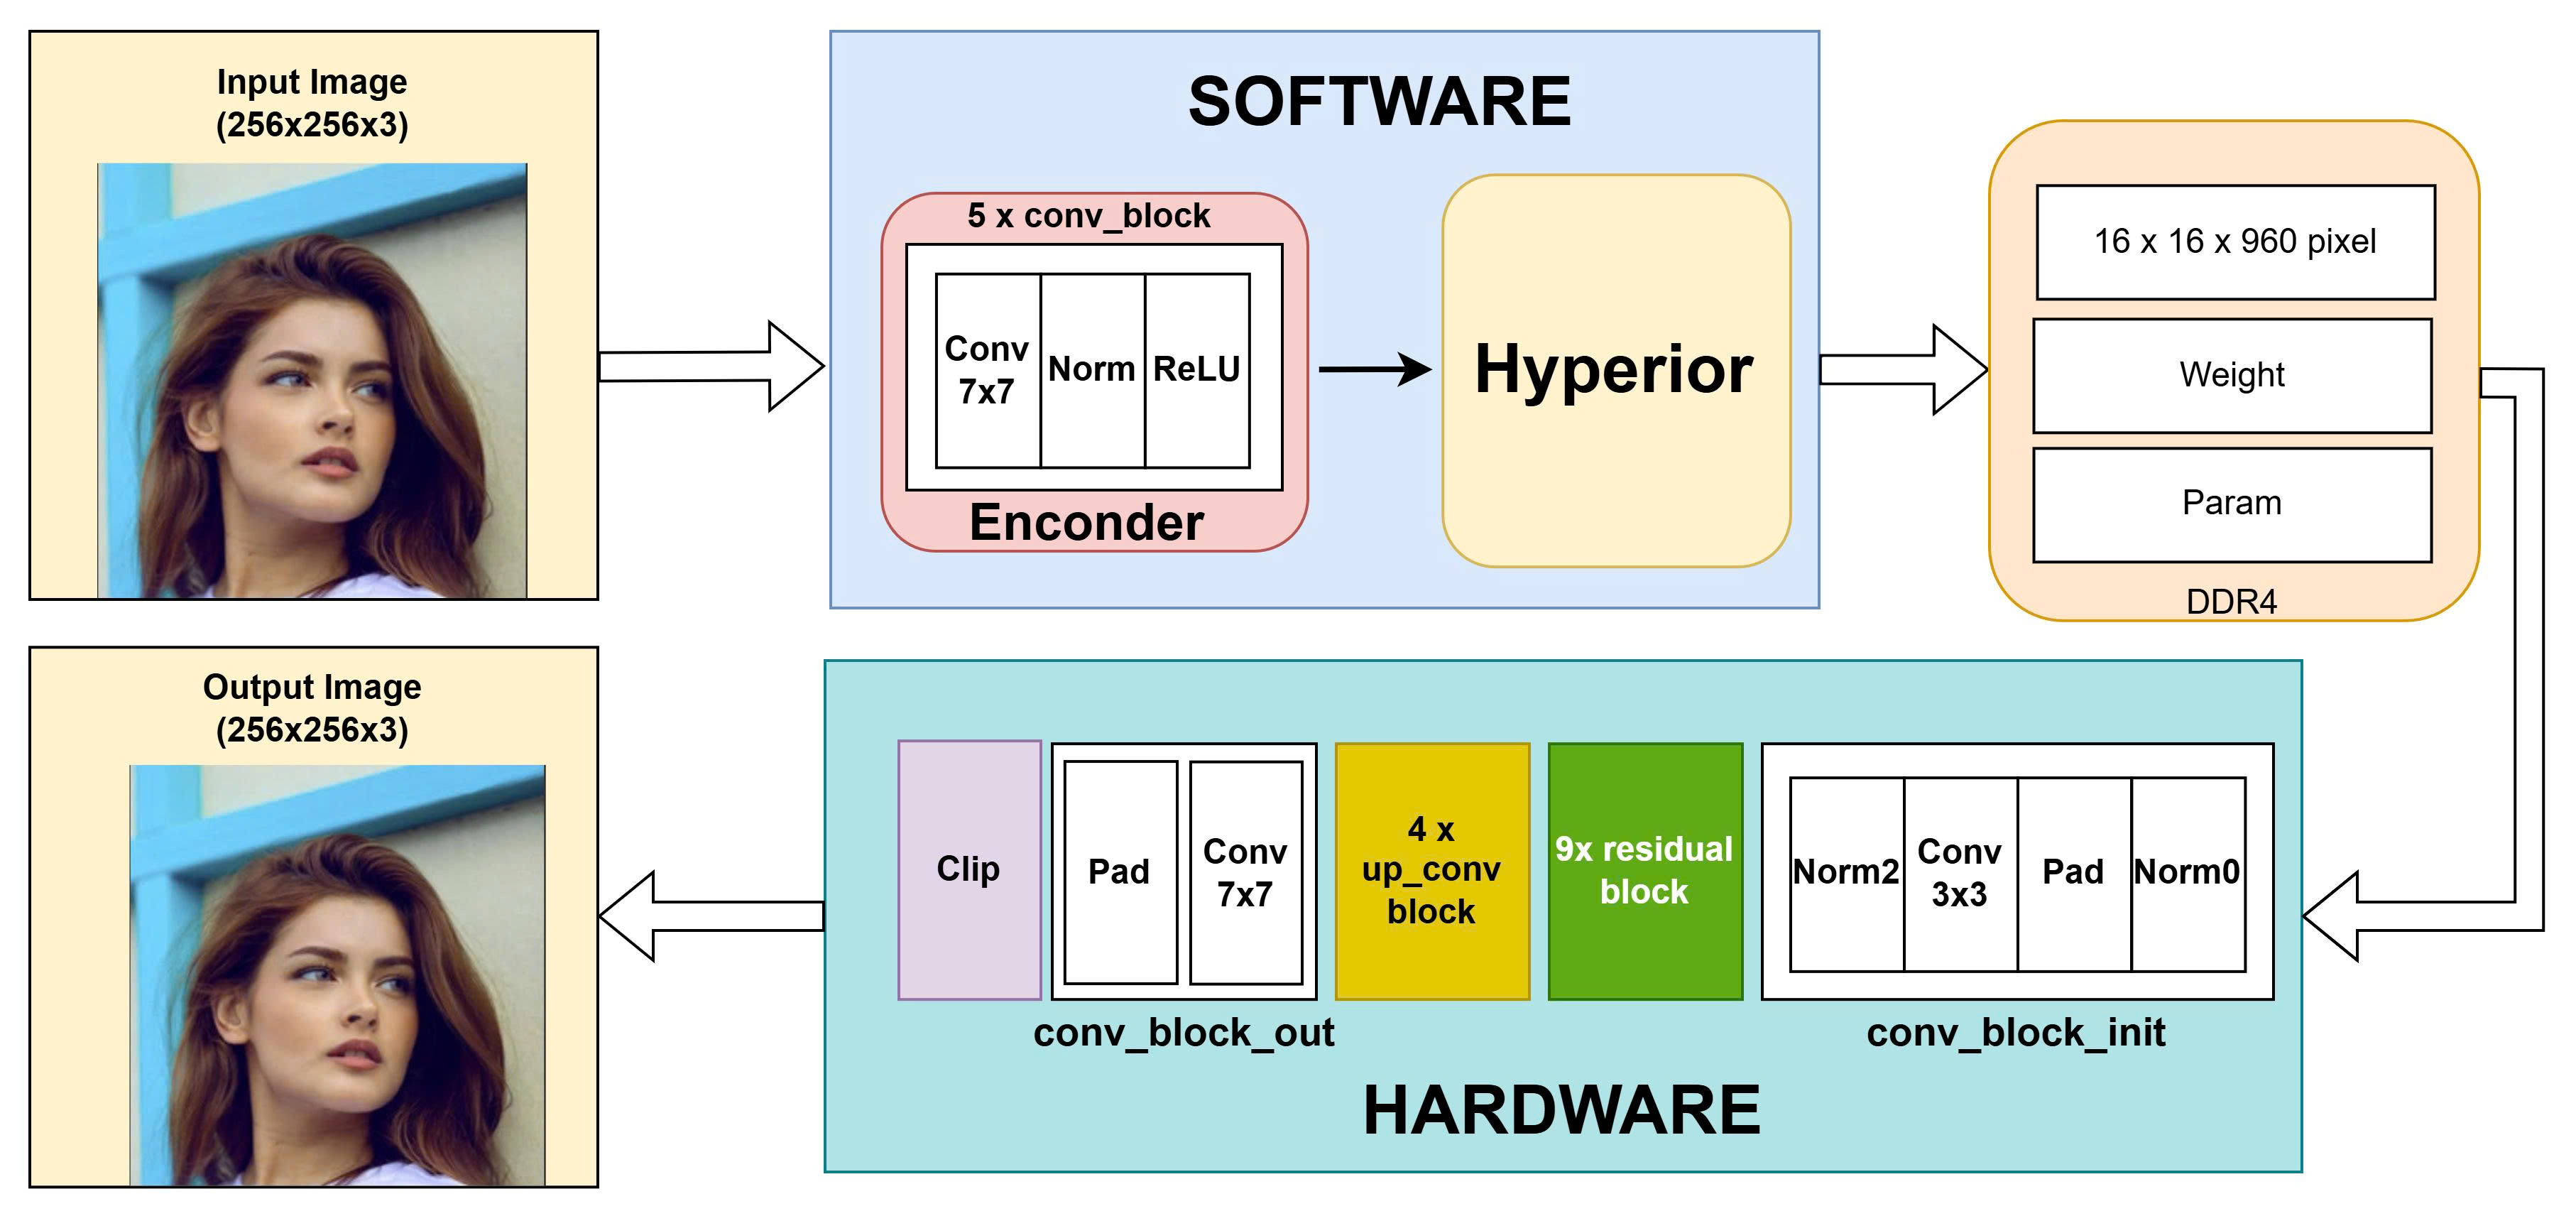
\includegraphics[width=1.0\textwidth]{Images/HW_SW.jpg}
    \caption{System-level hardware--software co-design overview of the HiFiC inference pipeline}
    \label{fig:hw_sw_overview}
\end{figure}

The PS--PL communication is organized through a small number of well-defined interfaces, as summarized in Table~\ref{tab:system_interfaces}. This interface view makes the system partition explicit and connects the high-level architecture in Figure~\ref{fig:hw_sw_overview} with the detailed ResBlock accelerator design presented later in this chapter.

\begin{table}[H]
\centering
\caption{System-level interfaces used by the ResBlock accelerator}
\label{tab:system_interfaces}
\begin{tabularx}{\textwidth}{|p{0.24\textwidth}|p{0.24\textwidth}|X|}
\hline
\textbf{Interface} & \textbf{Direction} & \textbf{Role in the system} \\
\hline
AXI4-Lite control & PS $\rightarrow$ PL & Transfers configuration values such as tensor dimensions, base addresses, start command, and status polling. \\
\hline
AXI master read & PL $\rightarrow$ DDR & Loads input feature maps, convolution weights, bias values, and normalization parameters from shared memory. \\
\hline
AXI master write & PL $\rightarrow$ DDR & Writes the output feature map of the accelerated ResBlock back to shared memory. \\
\hline
Shared DDR buffers & PS $\leftrightarrow$ PL & Provide the common storage space used to exchange large tensors between software execution and hardware acceleration. \\
\hline
\end{tabularx}
\end{table}

From the software perspective, each accelerator call behaves as a coarse-grained operation. The PS prepares the input and parameter buffers in DDR, writes the required configuration values through AXI4-Lite, starts the accelerator, waits for completion, and then continues with the remaining stages of the inference pipeline. From the hardware perspective, the PL only needs to implement a regular ResBlock datapath with memory-mapped input and output ports, which keeps the accelerator reusable across repeated residual blocks.

%%%%%%%%%%%%%%%%%%%%%%%%%%%%%%%%%%%%%%%%%%%%%%%%%%%%%%%%%%%%%%%%%%%%%%%%%%%%%%%%%%%%%%%%%%%%%%%%%%%%
\subsection{Mixed-Precision Quantization of HiFiC Model}

The deployment of learned image compression models such as HiFiC on FPGA platforms introduces significant challenges related to memory bandwidth, storage capacity, and computational efficiency. To address these constraints, a mixed-precision quantization strategy is adopted, aiming to reduce numerical precision while preserving compression performance and perceptual quality.

Figure~\ref{fig:quantize_arch_final_clean} illustrates the proposed quantization architecture applied to the HiFiC model. The quantization process is designed to operate in a post-training manner, eliminating the need for retraining and enabling rapid deployment on the target hardware.

\begin{figure}[H]
\centering
\begin{tikzpicture}[
    node distance=0.9cm and 2.6cm,
    every node/.style={font=\small},
    block/.style={
        rectangle,
        draw,
        rounded corners,
        align=center,
        minimum width=3.0cm,
        minimum height=0.85cm
    },
    smallblock/.style={
        rectangle,
        draw,
        rounded corners,
        align=center,
        minimum width=2.7cm,
        minimum height=0.75cm
    },
    arrow/.style={->, thick}
]

% ================= Left control path =================
\node[smallblock] (const) {ConstantOfShape};
\node[smallblock, below=of const] (concat) {Concat};
\node[smallblock, below=of concat] (reshape1) {Reshape};
\node[smallblock, below=of reshape1] (slice) {Slice};
\node[smallblock, below=of slice] (transpose) {Transpose};
\node[smallblock, below=of transpose] (reshape2) {Reshape};
\node[smallblock, below=of reshape2] (castL) {Cast to FP16};

% ================= Right data path =================
\node[block, right=of slice, xshift=2.4cm] (input) {Input Tensor\\FP32};
\node[smallblock, below=of input] (castR) {Cast to FP16};

% ================= Pad + Conv =================
\node[block, below=1.8cm of castR] (pad) {Pad};
\node[block, below=of pad] (conv) {Convolution Layer\\FP16};

% ================= Outputs =================
\node[smallblock, below left=1.2cm and 1.6cm of conv] (mean) {ReduceMean};
\node[smallblock, below right=1.2cm and 1.6cm of conv] (sub) {Sub};

% ================= Straight vertical arrows =================
\draw[arrow] (const) -- (concat);
\draw[arrow] (concat) -- (reshape1);
\draw[arrow] (reshape1) -- (slice);
\draw[arrow] (slice) -- (transpose);
\draw[arrow] (transpose) -- (reshape2);
\draw[arrow] (reshape2) -- (castL);

\draw[arrow] (input) -- (castR);

% ================= HARD ROUTED ORTHOGONAL MERGE =================

% Left Cast -> Pad (horizontal then vertical)
\coordinate (Lmid) at ($(castL.east)+(1.2,0)$);
\draw[arrow] (castL.east) -- (Lmid) |- (pad.west);

% Right Cast -> Pad (vertical straight)
\draw[arrow] (castR.south) -- (pad.north);

% ================= Downstream =================
\draw[arrow] (pad) -- (conv);

\coordinate (Cmid) at ($(conv.south)+(0,-0.7)$);
\draw[arrow] (conv.south) -- (Cmid) -| (mean.north);
\draw[arrow] (conv.south) -- (Cmid) -| (sub.north);

\end{tikzpicture}
\caption{Mixed-precision quantization architecture applied to convolutional layers}
\label{fig:quantize_arch_final_clean}
\end{figure}




\subsubsection{Quantization Strategy}

A post-training mixed-precision quantization approach is employed, where the internal computation of the neural network is performed using 16-bit floating-point (FP16) precision, while maintaining 32-bit floating-point (FP32) precision at the input and output interfaces. This strategy balances computational efficiency with numerical stability and compatibility with existing preprocessing and postprocessing pipelines.

The quantization strategy consists of the following key principles:
\begin{itemize}
    \item \textbf{Interface Preservation:} The input and output tensors of the HiFiC model remain in FP32 format to ensure compatibility with external modules.
    \item \textbf{Internal Precision Reduction:} All intermediate feature maps and arithmetic operations within the network are executed in FP16 precision.
    \item \textbf{Static Weight Casting:} Convolutional kernels, bias terms, and learned parameters are statically converted from FP32 to FP16 to reduce memory footprint.
\end{itemize}

To enforce this precision boundary, explicit casting operations are inserted immediately after the input layer (FP32 to FP16) and before the output layer (FP16 to FP32). Redundant casting operators introduced during automatic model conversion are identified and removed to maintain a continuous FP16 dataflow throughout the network.

\subsubsection{Operator-Level Precision Mapping}

Following quantization, the HiFiC model executes the majority of its operations within the FP16 domain. These operations can be categorized into two main groups:

\begin{itemize}
    \item \textbf{Computational Operations:} Convolution (Conv), transposed convolution (ConvTranspose), and matrix multiplication layers dominate the arithmetic workload of the Generator and are executed entirely in FP16 precision. This enables efficient utilization of FPGA DSP resources for multiply-accumulate (MAC) operations.
    \item \textbf{Non-linear and Element-wise Operations:} Activation functions (ReLU), element-wise addition, subtraction, multiplication, division, and exponential functions are also performed in FP16 precision, ensuring consistency across the computation graph.
\end{itemize}

By enforcing FP16 computation across all internal operators, the model achieves a significant reduction in memory bandwidth consumption and computational complexity, while preserving the structural integrity of the HiFiC architecture.

\subsubsection{Quantization Rationale}

The choice of FP16 precision is motivated by its favorable trade-off between numerical range and hardware efficiency. Compared to integer-based quantization schemes, FP16 offers higher dynamic range and improved stability for GAN-based architectures, where small numerical perturbations can otherwise lead to visible degradation in reconstructed images.

This mixed-precision quantization framework establishes a robust foundation for hardware acceleration of the HiFiC model on FPGA platforms, enabling efficient execution without compromising compression fidelity or perceptual quality.

%%%%%%%%%%%%%%%%%%%%%%%%%%%%%%%%%%%%%%%%%%%%%%%%%%%%%%%%%%%%%%%%%%%%%%%%%%%%%%%%%%%%%%%%%%%%%%%%%%%%
\subsection{Workload Analysis and Acceleration Target}

To determine the most suitable hardware acceleration target, the generator network was profiled on a CPU platform. The execution time of each generator block was measured on an Intel Core i9 processor operating at 2.2\,GHz. The results are summarized in Table~\ref{tab:runtime_breakdown}.

\begin{table}[H]
\centering
\caption{Runtime breakdown of HiFiC generator blocks executed on Intel Core i9 CPU @ 2.2\,GHz}
\label{tab:runtime_breakdown}
\begin{tabular}{|l|c|c|}
\hline
\textbf{Block Name} & \textbf{Execution Time (s)} & \textbf{Percentage (\%)} \\ \hline
conv\_block\_init & 23.139 & 2.16 \\ \hline
res\_block\_0 & 111.327 & 10.37 \\ \hline
res\_block\_1 & 102.859 & 9.58 \\ \hline
res\_block\_2 & 97.376 & 9.07 \\ \hline
res\_block\_3 & 96.871 & 9.03 \\ \hline
res\_block\_4 & 96.799 & 9.02 \\ \hline
res\_block\_5 & 102.545 & 9.55 \\ \hline
res\_block\_6 & 106.396 & 9.91 \\ \hline
res\_block\_7 & 113.640 & 10.59 \\ \hline
res\_block\_8 & 118.866 & 11.08 \\ \hline
upconv\_blocks (Total 1--4) & 87.696 & 8.17 \\ \hline
conv\_block\_out & 15.588 & 1.45 \\ \hline
Others (Add, Overhead) & 0.088 & 0.03 \\ \hline
\textbf{Total Runtime} & \textbf{1073.19} & \textbf{100} \\ \hline
\end{tabular}
\end{table}

The profiling result shows that the residual blocks dominate the generator runtime. Together, the repeated ResBlocks account for more than 78\% of the total execution time, while the initial convolution, up-convolution blocks, and output convolution occupy a much smaller share. This makes the ResBlock the most effective target for acceleration.

The ResBlocks are also attractive from a hardware design perspective because they share a regular computation pattern. Each block is mainly composed of convolution, normalization, activation, and residual addition. The convolution layers reuse the same local-window structure across many spatial positions and channels, which matches the strengths of FPGA architectures: local buffering, parallel MAC units, and pipelined execution.

In this implementation, the accelerator focuses on the repeated ResBlock computation inside the generator. Other parts of the HiFiC pipeline remain in software to reduce design complexity and preserve flexibility. This scope allows the hardware design to concentrate resources on the block that provides the greatest latency reduction.

%%%%%%%%%%%%%%%%%%%%%%%%%%%%%%%%%%%%%%%%%%%%%%%%%%%%%%%%%%%%%%%%%%%%%%%%%%%%%%%%%%%%%%%%%%%%%%%%%%%%
\subsection{Detailed Internal Block Design}

This section describes the main internal blocks used to implement the ResBlock accelerator. Similar to the structure of a standard implementation chapter, the explanation starts from data buffering, then moves to the processing element architecture, the full ResBlock datapath, and the execution schedule.

\subsubsection{Line Buffer, Window, and Boundary Handling}

The ResBlock accelerator processes convolution windows in a streaming manner. Instead of repeatedly loading the same pixels or feature values from external memory, the design stores recently used rows in on-chip line buffers. For a $3 \times 3$ convolution, two previous rows are sufficient because the current row is provided by the input stream.

\begin{figure}[H]
    \centering
    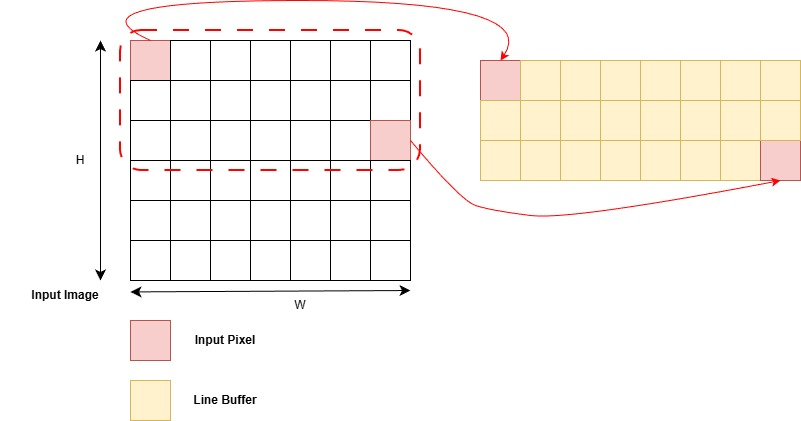
\includegraphics[width=0.8\textwidth]{Images/Line Buffer.jpg}
    \caption{Two-line buffer structure for streaming convolution}
    \label{fig:line_buffer_structure}
\end{figure}

Figure~\ref{fig:line_buffer_structure} illustrates the two-line buffer organization. As new feature values arrive in raster-scan order, the buffer keeps the spatial relationship between adjacent rows. This allows the accelerator to construct valid convolution windows without reloading the same rows from DDR memory.

\begin{figure}[H]
    \centering
    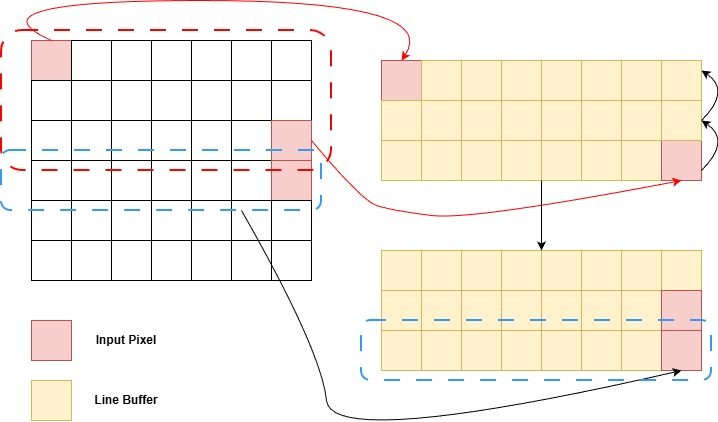
\includegraphics[width=0.8\textwidth]{Images/Line buffer flow.jpg}
    \caption{Two-line buffer dataflow and update mechanism}
    \label{fig:line_buffer_flow}
\end{figure}

The update behavior is shown in Figure~\ref{fig:line_buffer_flow}. At each new input position, stored values are shifted to keep the previous rows aligned with the current row. This structure converts external memory traffic into local buffer reuse, which is essential for high-throughput convolution on FPGA.

\begin{figure}[H]
    \centering
    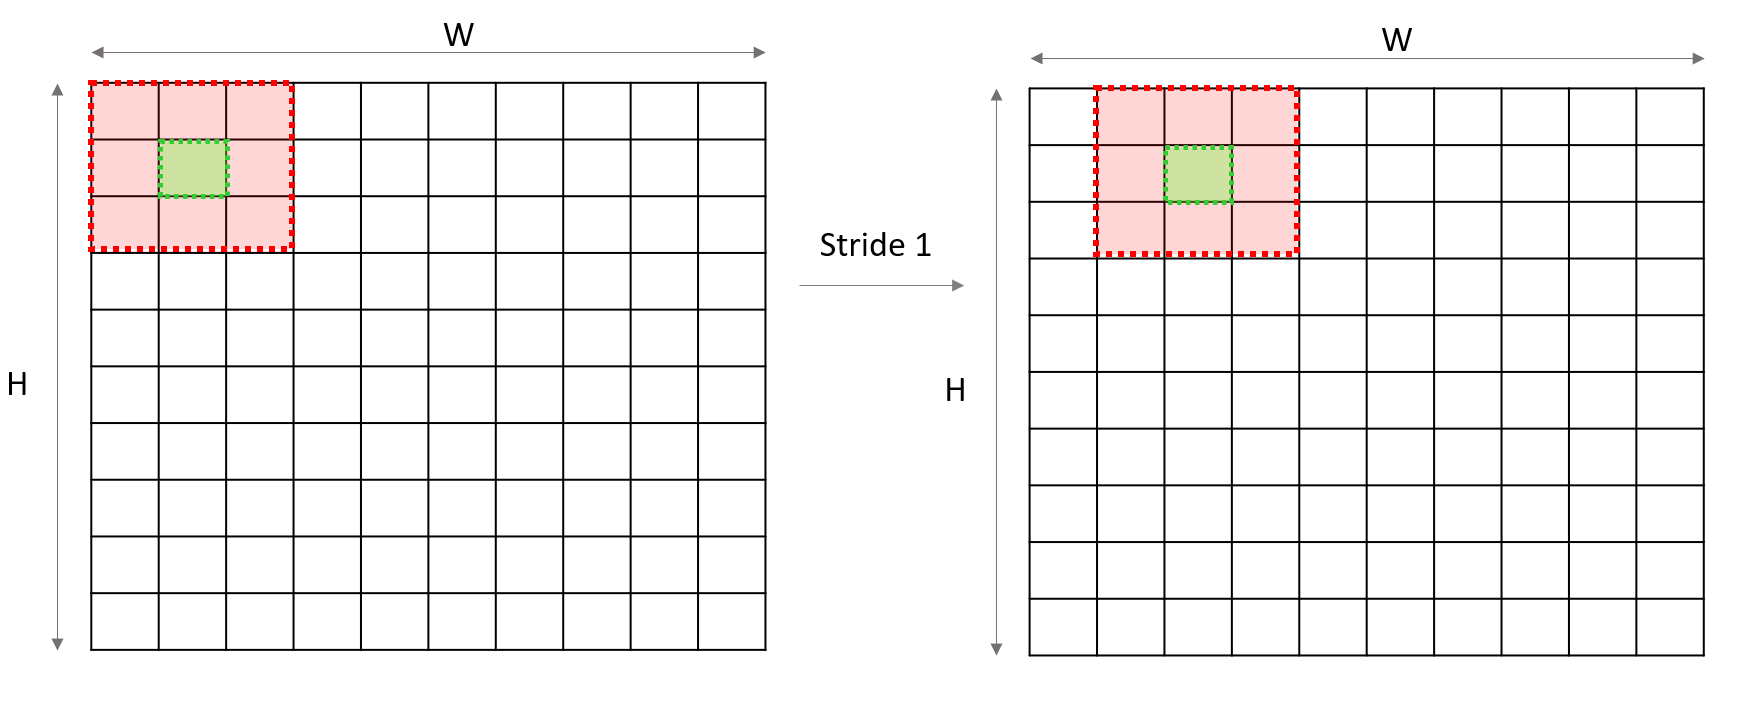
\includegraphics[width=0.6\textwidth]{Images/window.png}
    \caption{Sliding window structure for convolution processing}
    \label{fig:sliding_window}
\end{figure}

After the line buffer prepares neighboring rows, a sliding window extracts the local $3 \times 3$ region required by each convolution operation. The window structure in Figure~\ref{fig:sliding_window} provides the input values for the PE cluster. In the proposed design, multiple window positions on the same row can be generated in parallel so that several output pixels are computed at the same time.

\begin{figure}[H]
    \centering
    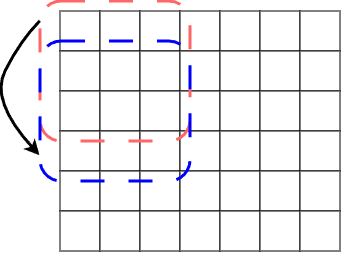
\includegraphics[width=0.6\textwidth]{Images/Window Data Update.drawio.png}
    \caption{Parallel window update mechanism with vertical-only movement}
    \label{fig:window_update}
\end{figure}

Figure~\ref{fig:window_update} shows the window update mechanism used to support parallel processing. Rather than moving a single window across the row one position at a time, the architecture assigns multiple horizontal positions to different processing lanes. The input stream then advances to the next row, while each lane maintains the correct local neighborhood for its assigned output position.

Boundary handling is implemented using reflection padding, as shown in Figure~\ref{fig:reflection_padding}. Reflection padding mirrors feature values at the border, preserving local continuity near image boundaries. This is suitable for image reconstruction workloads because it avoids the abrupt border discontinuities that may be introduced by simple zero padding.

\begin{figure}[H]
    \centering
    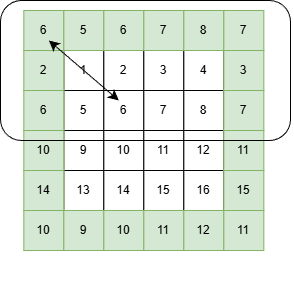
\includegraphics[width=0.6\textwidth]{Images/Reflect Pad.png}
    \caption{Reflection padding used in the generator network}
    \label{fig:reflection_padding}
\end{figure}

\subsubsection{Processing Element Architecture}

The Processing Element (PE) is the basic arithmetic unit of the accelerator. Each PE computes one convolution result by multiplying input feature values with the corresponding kernel weights and accumulating the products.

\begin{figure}[H]
    \centering
    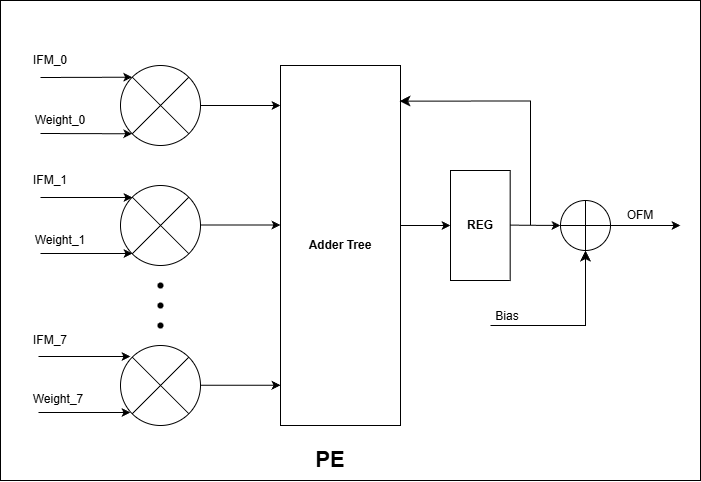
\includegraphics[width=0.7\textwidth]{Images/PE.png}
    \caption{Processing Element (PE) architecture for convolution computation}
    \label{fig:pe_architecture}
\end{figure}

As shown in Figure~\ref{fig:pe_architecture}, the PE contains parallel multipliers, an adder tree, pipeline registers, and bias addition. The multipliers are mapped to FPGA DSP resources, while the adder tree reduces the partial products with low latency. Pipeline registers are inserted to support continuous operation and improve timing closure.

Multiple PEs are instantiated to form a PE cluster. Each PE is assigned to a different spatial window or output lane. This organization increases throughput by computing several convolution outputs in parallel and by reusing the same buffered input data across multiple lanes.

\subsubsection{ResBlock Accelerator Architecture}

The computational structure of a generator ResBlock is shown in Figure~\ref{fig:resblock_flow}. A ResBlock applies convolutional transformations to the input feature map and combines the processed result with the original input through a skip connection. This residual path helps preserve important feature information while allowing the convolution path to refine texture and detail.

\begin{figure}[H]
    \centering
    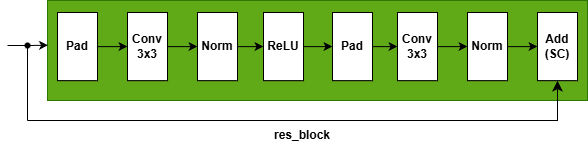
\includegraphics[width=1.0\textwidth]{Images/resblock.png}
    \caption{Computational flow of a ResBlock in the HiFiC generator}
    \label{fig:resblock_flow}
\end{figure}

The proposed hardware architecture for this block is presented in Figure~\ref{fig:resblock_architecture}. The accelerator contains input feature buffering, weight buffering, window generation, a PE cluster, output feature buffering, normalization and activation logic, and a skip-connection buffer. These blocks cooperate to execute the full ResBlock while minimizing off-chip memory traffic.

\begin{figure}[H]
    \centering
    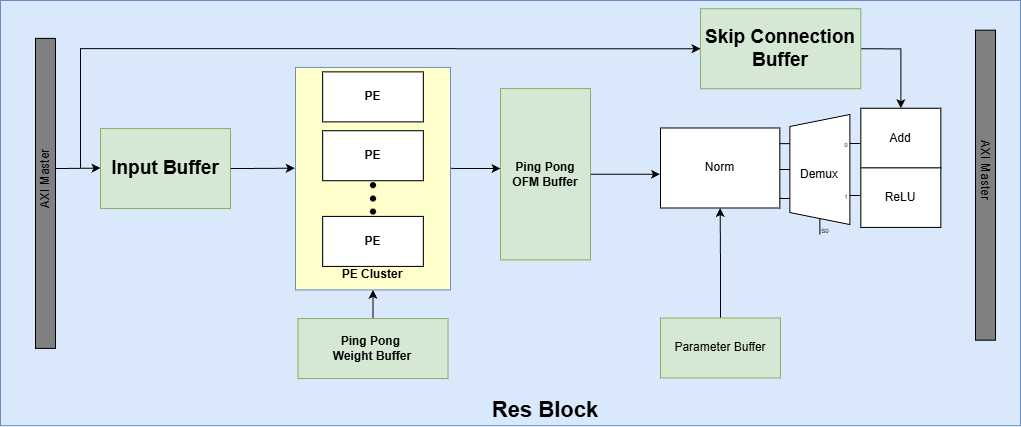
\includegraphics[width=0.98\textwidth]{Images/Resblock Hardware Architecture.png}
    \caption{Proposed hardware architecture of the ResBlock accelerator}
    \label{fig:resblock_architecture}
\end{figure}

The input feature buffer stores the feature values required by the line buffer and window generation logic. The weight buffer stores convolution kernels so that they can be reused across spatial positions without repeated DDR accesses. The residual buffer preserves the original input feature map until the final residual addition is performed. The output feature buffer temporarily stores intermediate results between the convolution and post-processing stages.

\subsubsection{Two-Pass Execution Strategy}

The ResBlock contains multiple computation stages, but implementing every stage as a separate hardware core would increase resource usage and interface complexity. To avoid this, the accelerator uses a two-pass execution strategy, shown in Figure~\ref{fig:two_pass_architecture}.

\begin{figure}[H]
    \centering
    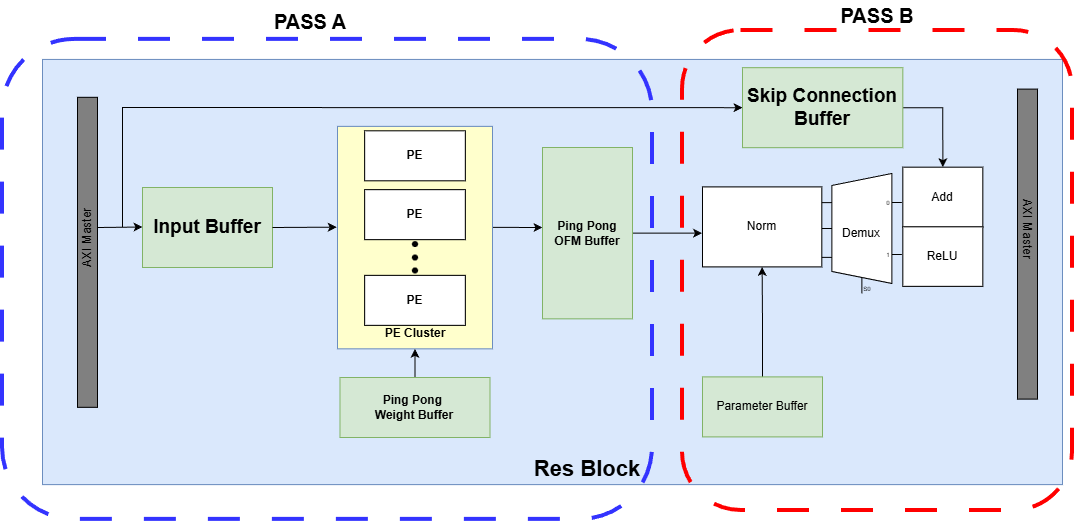
\includegraphics[width=1.0\textwidth]{Images/Two Pass architecture.png}
    \caption{Two-pass execution architecture of the ResBlock accelerator}
    \label{fig:two_pass_architecture}
\end{figure}

In the first pass, the accelerator performs the first convolution and writes the intermediate feature map into the output feature buffer. Normalization and activation are applied before the intermediate result is forwarded to the second pass. In the second pass, the accelerator performs the next convolution, applies the remaining post-processing, and combines the result with the stored skip connection to generate the final output feature map.

This execution strategy reuses the same PE cluster for both convolution stages, which reduces hardware duplication. It also keeps intermediate data on chip whenever possible, decreasing external memory traffic and improving latency.

\begin{figure}[H]
    \centering
    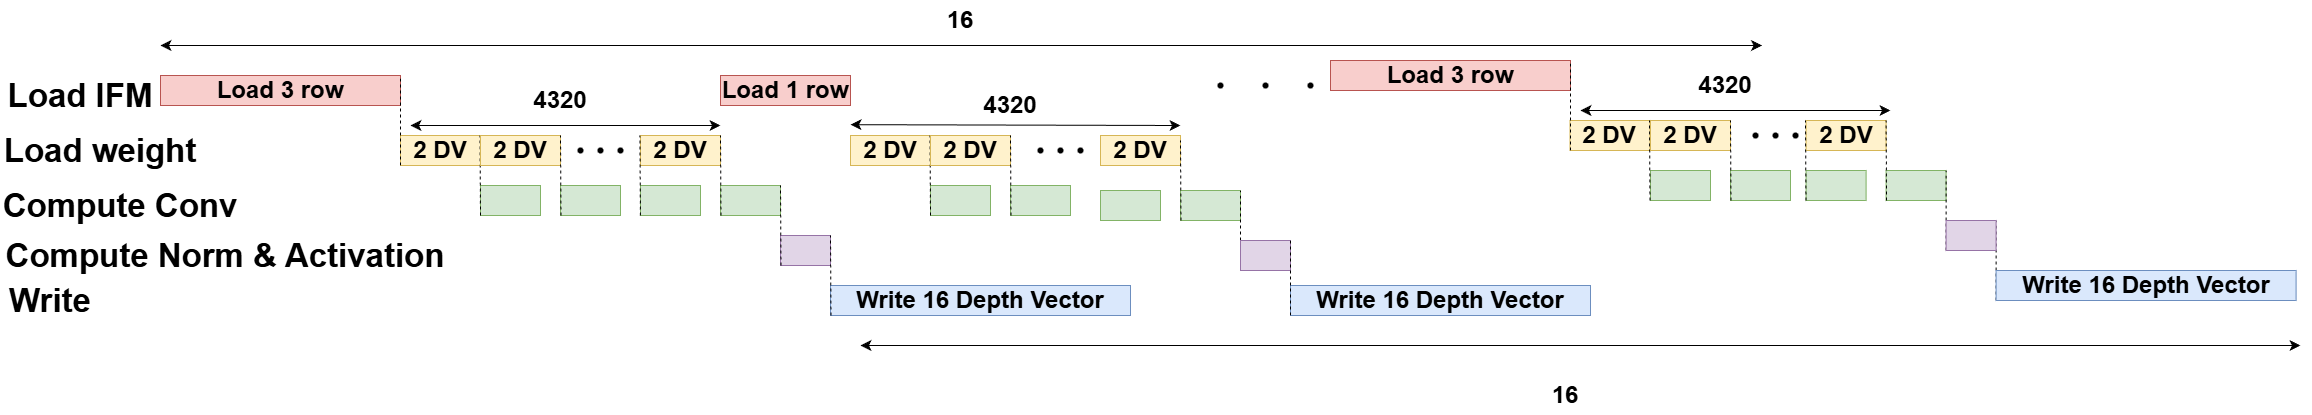
\includegraphics[width=0.95\textwidth]{Images/Pipeline Timing.png}
    \caption{Pipeline timing diagram of the proposed ResBlock accelerator}
    \label{fig:pipeline_timing}
\end{figure}

Figure~\ref{fig:pipeline_timing} illustrates the overlapped schedule of loading, computation, post-processing, and output writing. After the initial warm-up period, the pipeline reaches a steady state where different rows are processed by different stages at the same time. This overlap is a key factor in reducing the total execution time of the ResBlock accelerator.

\subsubsection{Top-Level Kernel Interface}

The HLS kernel exposes a memory-mapped interface that allows the PS to configure and invoke the accelerator. The top-level design uses AXI master ports for large tensors and parameter arrays, and an AXI4-Lite control interface for scalar configuration values and start/done synchronization.

The main interface groups are:
\begin{itemize}
    \item \textbf{Input feature map port:} reads the feature tensor of the current ResBlock from external DDR memory.
    \item \textbf{Weight and parameter ports:} load convolution kernels, bias values, and normalization parameters required by the block.
    \item \textbf{Output feature map port:} writes the final ResBlock output back to DDR memory.
    \item \textbf{Control port:} receives tensor dimensions, memory offsets, start signals, and status flags from the PS.
\end{itemize}

This interface makes the accelerator reusable across repeated ResBlocks. The PS can invoke the same hardware kernel multiple times with different memory addresses and parameters, while the internal datapath remains unchanged.

%%%%%%%%%%%%%%%%%%%%%%%%%%%%%%%%%%%%%%%%%%%%%%%%%%%%%%%%%%%%%%%%%%%%%%%%%%%%%%%%%%%%%%%%%%%%%%%%%%%%
\subsection{High-Level Synthesis and FPGA Deployment}

High-Level Synthesis is used to transform the C/C++ accelerator description into RTL hardware. This approach reduces design time compared with writing the complete datapath manually in Verilog or VHDL, while still allowing hardware-specific optimization through HLS directives.

\begin{figure}[H]
    \centering
    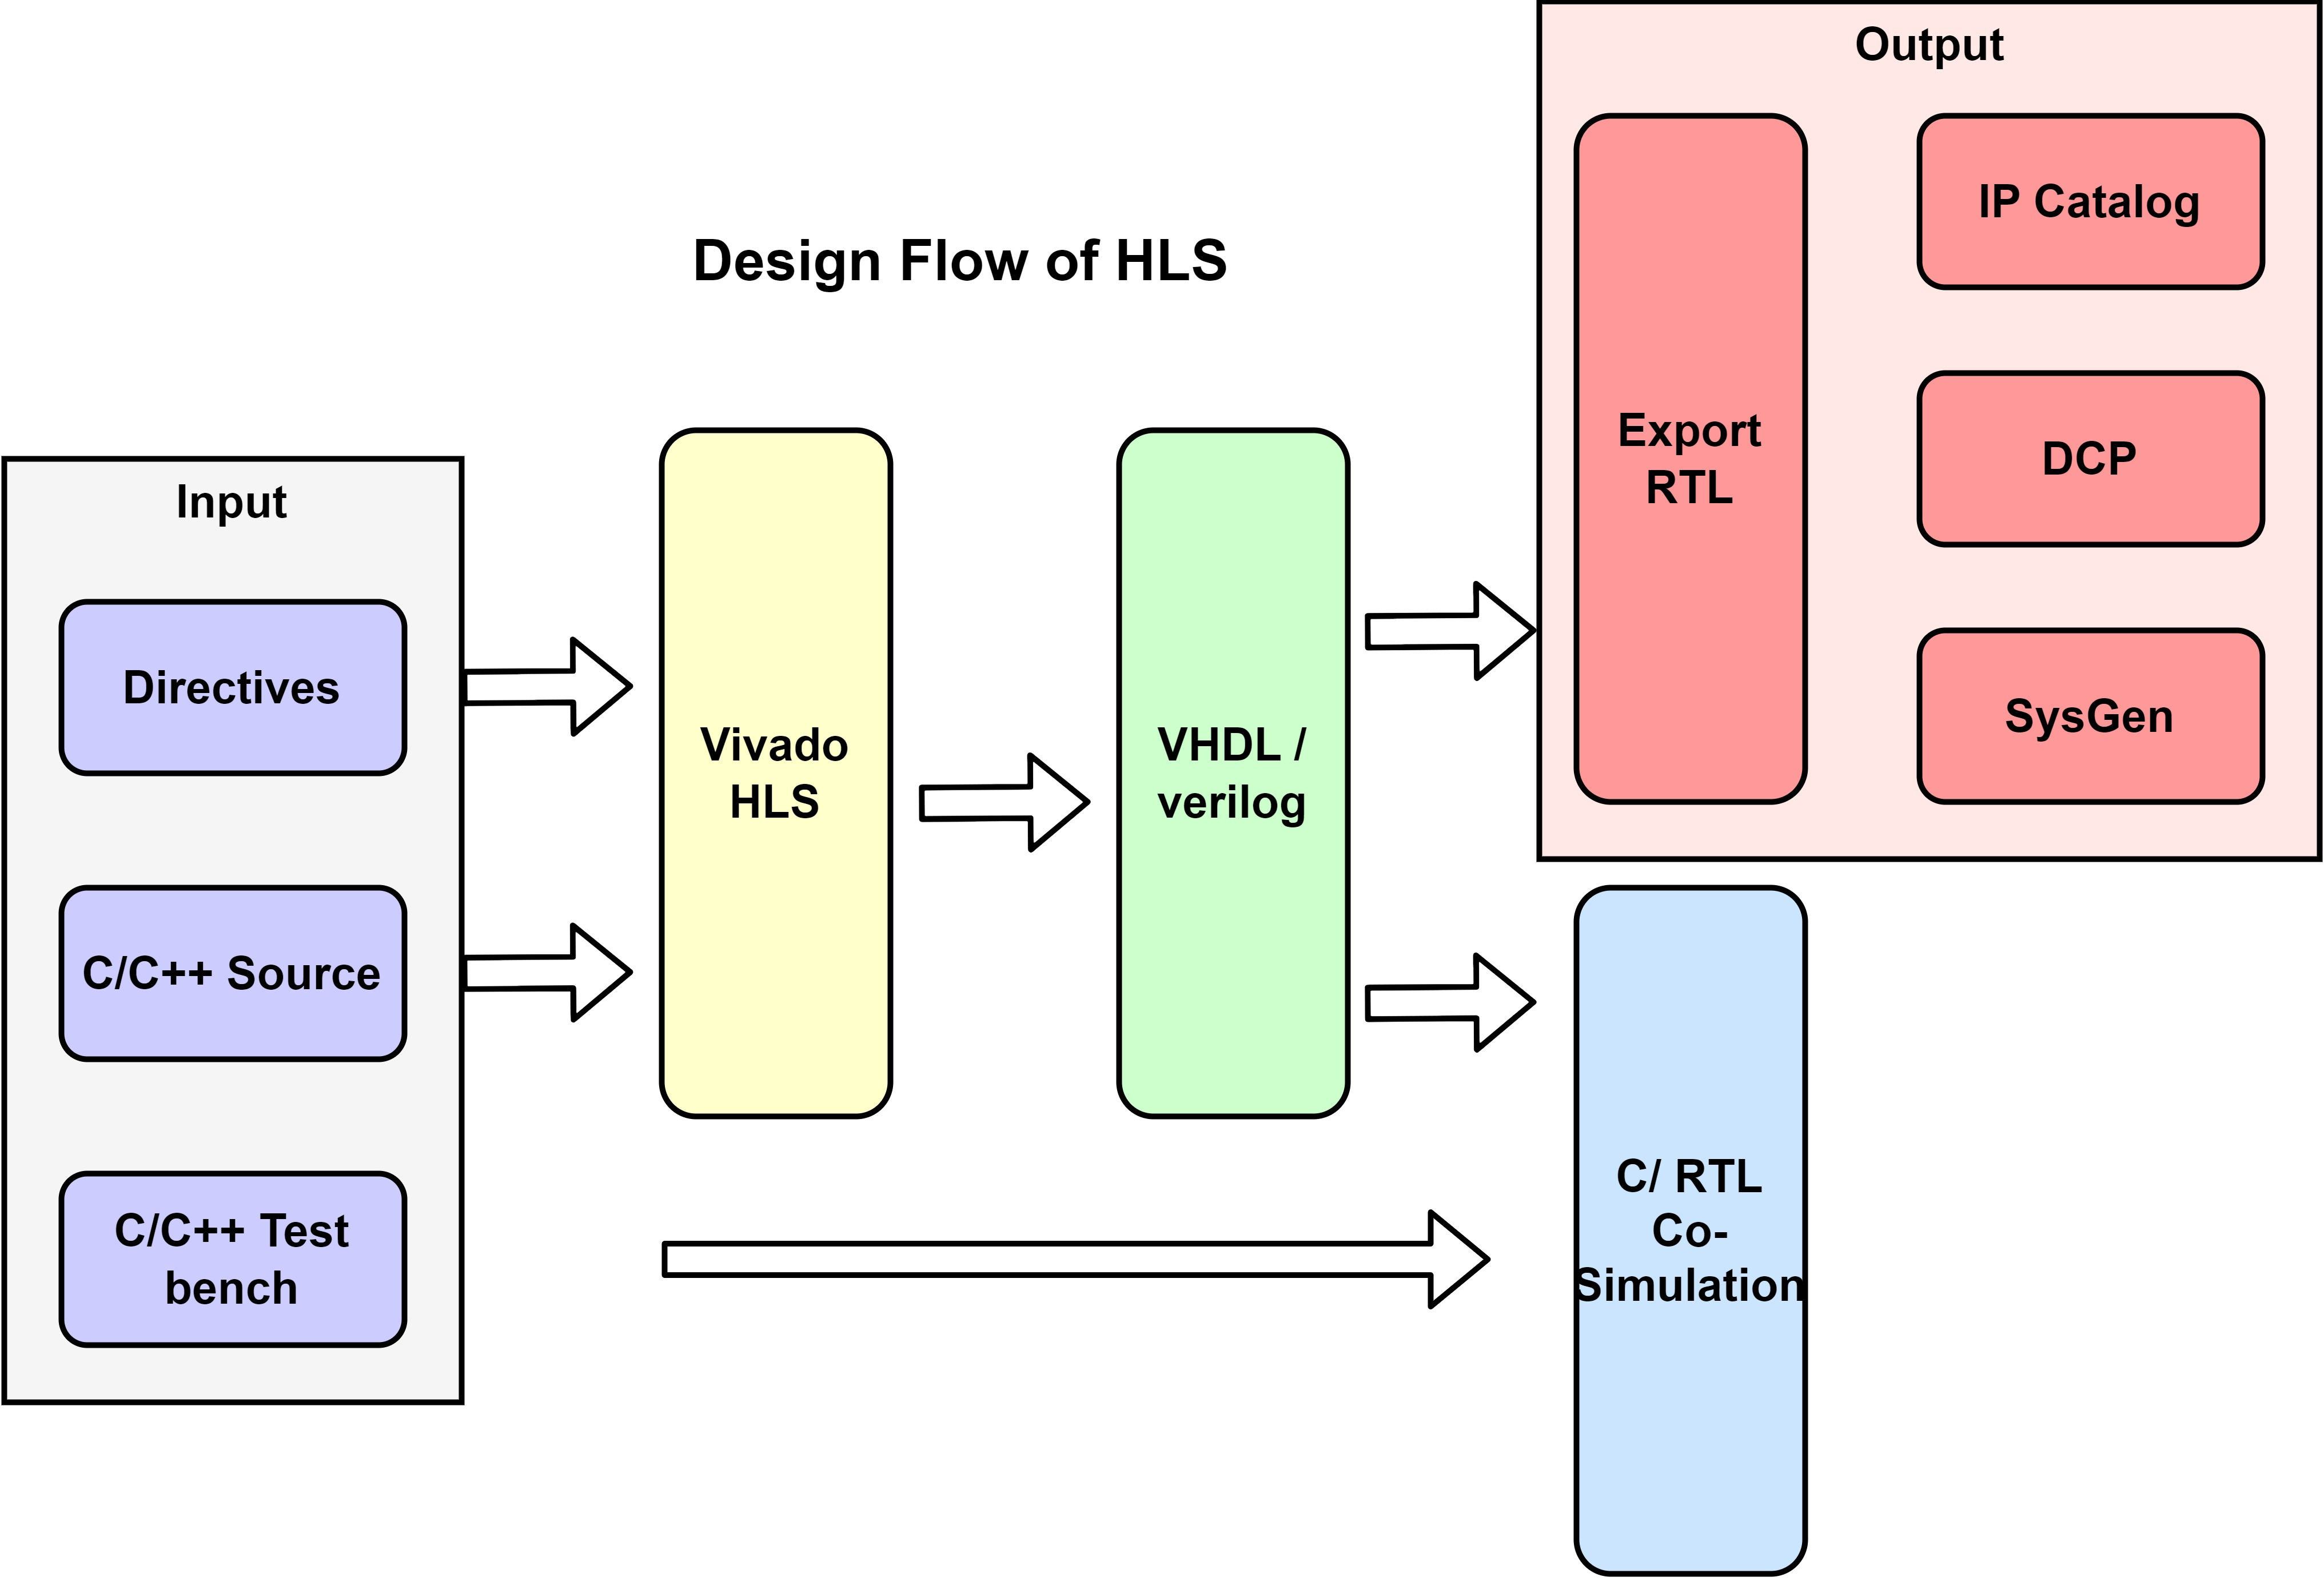
\includegraphics[width=0.8\textwidth]{Images/flow_LSI-Page-9.jpg}
    \caption{High-Level Synthesis design flow}
    \label{fig:hls_design_flow}
\end{figure}

The deployment flow in Figure~\ref{fig:hls_design_flow} consists of C/C++ design, functional simulation, synthesis, RTL export, Vivado integration, and board-level execution. During C/C++ simulation, the accelerator output is compared with the software reference to verify functional correctness. After synthesis, Vitis HLS reports latency estimates, initiation intervals, and resource usage, which are used to refine the architecture.

Several HLS techniques are applied in the implementation:
\begin{itemize}
    \item \textbf{Loop pipelining:} overlaps loop iterations so that new data can enter the datapath every cycle or after a short initiation interval.
    \item \textbf{Array partitioning:} increases memory bandwidth for frequently accessed buffers such as windows, weights, and partial sums.
    \item \textbf{Dataflow scheduling:} enables loading, computation, and output writing functions to execute concurrently.
    \item \textbf{Interface directives:} map large data arrays to AXI master ports and scalar control values to AXI4-Lite registers.
\end{itemize}

After the accelerator is exported as an IP core, Vivado is used to connect it with the Zynq Processing System, AXI interconnects, DDR memory, clocking, and reset logic. The final bitstream configures the PL with the ResBlock accelerator. On the software side, a Vitis application running on the ARM processor prepares input buffers, writes configuration registers, launches the accelerator, and reads back the output data for the remaining inference stages.

This implementation flow provides a complete path from neural network analysis to executable FPGA deployment. It also separates architectural design decisions in this chapter from the resource, timing, and performance evaluation reported in the following chapters.

%%%%%%%%%%%%%%%%%%%%%%%%%%%%%%%%%%%%%%%%%%%%%%%%%%%%%%%%%%%%%%%%%%%%%%%%%%%%%%%%%%%%%%%%%%%%%%%%%%%%
\subsection{Chapter Conclusion}

This chapter presented the implementation architecture of the HiFiC GAN accelerator. The system was organized as a hardware--software co-design in which the PS handles control and flexible processing, while the PL accelerates the repeated ResBlock computation in the generator network.

The chapter also described the internal accelerator blocks, including line buffers, sliding windows, reflection padding, PE clusters, on-chip buffers, and the two-pass ResBlock execution strategy. Finally, the HLS and FPGA deployment flow was introduced to show how the C/C++ design is synthesized, integrated, and controlled on the ZCU104 platform. The next chapter evaluates the resulting FPGA implementation in terms of resource utilization, system integration, and performance.